\chapter{Projektstruktur und -organisation}
\label{sec:orga}
\marginpar{Benjamin}

In der ersten Woche der Projektgruppe wurde eine Seminarphase durchgeführt, in
der die theoretischen Grundlagen des Themas sowie Grundlagen des
Projektmanagements und der Softwareentwicklung erarbeitet wurden. Im Anschluss wurde in
der Projektgruppenordnung festgehalten, wie die Projektgruppe weiter verlaufen
wird. In der Seminarphase stellten sich folgende Tools als besonders geeignet
heraus, um den weiteren Ablauf der Projektgruppe zu organisieren:

\begin{itemize}
    \item \qmarks{Scrum} als Vorgehensmodell für die Projektgruppe.
    \item \qmarks{Redmine} als Ticketsystem zur Verwaltung der Aufgaben und deren
      Verteilung, sowie als Wiki zum Festhalten von Protokollen und
      organisatorischen Informationen.
    \item \qmarks{Git} als Versionskontrolle und zur Verwaltung des Quellcodes.
\end{itemize}

\section{Projektmanagement}
\label{sec:orga:projekt}
\marginpar{Benjamin}

Im Projektmanagement kommt es vor allen Dingen auf klare
Aufgabendefinitionen und das Setzen eindeutiger Start- und Endtermine an. Die Ziele der Projektgruppe stehen im Vordergrund und müssen klar
strukturiert und verständlich aufgeschlüsselt werden, sodass ein
funktionierendes Miteinander gewährleistet ist. Um das Ziel der Projektgruppe zu erreichen, müssen die Bestimmungsgrößen \qmarks{Ziel}, \qmarks{Zeit} und \qmarks{Ressourcen} entsprechend
heruntergebrochen werden, um Teilaufgaben auf die Teilnehmer zu verteilen.
% Anm. Marcel: was muss wie genau verteilt werden? Sind Teilaufgaben gemeint? Anm. Jan: Ich würde sagen, ja. Habs jetzt mal geändert, ansonsten Benjamin, bitte wieder zurückändern.
Standardvorgehensmodelle bieten einen gewissen Aufbau, mit dem sich die
Projektgruppe gezielt organisieren kann. Die Projektgruppe identifizierte jedoch
auch gewisse Kernelemente, die auch über das Vorgehensmodell hinaus Geltung
finden. Diese Elemente sind:

\begin{itemize}
  \item Verwaltung und Identifizierung der Arbeitsschritte
  \item Gezieltes Aufteilen in klare, verständliche Arbeitspakete
  \item Effiziente Arbeits- und Arbeitslastenverteilung
  \item Rege Kommunikation
  \item Transparenz: Offenes Kommunizieren der Fähigkeiten und des Fortschritts
  \item Fortlaufende Dokumentation
\end{itemize}

\subsection{Rollen der Projektteilnehmer}
\label{sec:orga:projekt:rollen}
\marginpar{Benjamin}

In der Projektgruppenordnung wurden vier spezielle Rollen festgeschrieben und mit jeweils einer Person besetzt. Dabei handelt es sich um den

\begin{description}
\item[Projektleiter,] der die Verantwortung für das Projekt übernimmt und die
Arbeitsfortschritte überwacht. Er leitet jede Sitzung der Projektgruppe und
achtet auf die Einhaltung der Tagesordnung. Der Projektleiter übernimmt außerdem
die Aufgaben eines \textit{ScrumMasters}, der die wöchentlichen Fortschrittsberichte
koordiniert. Bei Abstimmungen mit Stimmengleichheit entscheidet der
Projektleiter.

\item[Protokollant,] der über jede Sitzung ein Protokoll führt. Dieses wird im
Redmine-Wiki hinterlegt und enthält die Namen der Anwesenden, die wesentlichen Inhalte der
Tagesordnungspunkte, Informationen zu eventuell abgehaltenen Abstimmungen und
sonstige abgegebene Erklärungen.

\item[Teamleiter,] der Tickets im Redmine erstellt und zuweist. Darüber hinaus
kümmert er sich um die Administration des Redmine-Systems.

\item[Berichtmanager,] der für die Einhaltung von Deadlines sorgt, die den Bericht
betreffen. Außerdem erstellt er Vorlagen und sichert die Qualität des Berichts durch
Einhaltung von formalen und inhaltlichen Kriterien.
\end{description}

\subsection{Scrum}
\label{sec:orga:projekt:scrum}
\marginpar{Benjamin}

Das Projektmanagement für die Projektgruppe lehnt sich an das Scrum-Framework
an. \textit{Scrum} ist ein agiles Vorgehensmodell zur Softwareentwicklung, in dem der
Zeitraum in Sprints aufgeteilt wird. Diese Sprints sind maximal einen Monat
lang und sorgen für eine inkrementelle Erweiterung des Projekts.

\begin{itemize}
\item Transparenz: Der Projektfortschritt wird in \textit{daily scrums} jeden
  Tag (\bzw jede Sitzung) für jedes Teammitglied sichtbar festgehalten.
\item Überprüfung: Durch die Sprints wird in regelmäßigen Abständen ein Ergebnis
  erzielt und am Ende eines Sprints kann dieser von den Teammitgliedern bewertet
  werden.
\item Anpassung: Die Planung wird kontinuierlich erweitert und verbessert.
\end{itemize}

In der Projektgruppe wird der Projektfortschritt wöchentlich besprochen, der
Projektleiter organisiert dies. Wir haben des Weiteren die zwei Semester der
Projektgruppe in insgesamt fünf Sprints aufgeteilt, die jeweils $5-7$ Wochen lang
sind.

\begin{figure}[htb]
\begin{center}
\begin{ganttchart}{1}{12}
\gantttitle{2014}{9}
\gantttitle{2015}{3} \\
\gantttitlelist{4,...,12,1,2,3}{1} \\
\ganttbar{Sprint 1}{1}{2} \\
\ganttbar{Sprint 2}{3}{4} \\
\ganttbar{Sprint 3}{7}{8} \\
\ganttbar{Sprint 4}{9}{10} \\
\ganttbar{Sprint 5}{11}{12}
\ganttlink{elem0}{elem1}
\ganttlink{elem1}{elem2}
\ganttlink{elem2}{elem3}
\ganttlink{elem3}{elem4}
\end{ganttchart}
\end{center}
\caption{Übersicht Sprintplanung}
\label{fig:sprintplanung}
\end{figure}

\begin{description}
  \item[1. Sprint] (6 Wochen) dient der Aneignung von theoretischem Vorwissen, des
    Herausarbeitens der Programmstruktur, der Auswahl der einzusetzenden Algorithmen
    sowie der Implementierung eines einfachen Prototypen, aus dem
    unser Readmapper dann weiterentwickelt werden kann.
  \item[2. Sprint] (7 Wochen) beinhaltet die Implementierung des Readmappers und die
    Erstellung des Zwischenberichts. Auf diesen Sprint folgt mit der
    vorlesungsfreien Zeit eine längere Pause.
  \item[3. Sprint] (6 Wochen) soll zur Ausführung von Benchmarks genutzt werden.
    Weiterführend soll das
    Finden neuer Varianten implementiert sowie eine grafische Oberfläche für
    unser Programm entworfen werden.
  \item[4. Sprint] (5 Wochen) ist gedacht für weitergehende Experimente und den
    Beginn der Auswertung.
  \item[5. Sprint] (5 Wochen) umfasst die finale Auswertung und Erstellung des Endberichts.
\end{description}

\subsection{Redmine}
\label{sec:orga:projekt:redmine}
\marginpar{Benjamin}

Zur Organisation wurde die Redmine-Installation des ITMC benutzt. Die
wesentlichen genutzten Funktionen dieses Systems sind Folgende: Im Wiki wird die
laufende Dokumentation der Projektgruppe festgehalten. Dies umfasst die
wöchentlichen Protokolle, die Projektgruppenordnung und Informationen zur
verwendeten Literatur. Im Ticketsystem wird dokumentiert, welche Aufgaben von
wem wann bearbeitet werden sollen. Dazu kann auch eine Kalenderansicht
aufgerufen werden, in der die Tickets zeitlich dargestellt werden. Des Weiteren
bietet Redmine ein Webinterface zur Ansicht der Änderungen in einem verknüpften
Git-Repository. Tickets und Änderungen im Git können sich gegenseitig
referenzieren. Das Redmine-System wird vom Teamleiter gepflegt, insbesondere
sorgt er für eine regelmäßige Aktualisierung der Tickets.

\section{Versionsverwaltung mit Git}
\label{sec:orga:vers}
\label{sec:orga:vers:git}
\marginpar{Kada}

Git ist ein Versionierungstool zur Codeverwaltung. Es wurde von Linus Torvalds aufgrund der Unzufriedenheit über die bisherigen Versionierungstools ins Leben gerufen. Das zuvor vom Linux-Kernel verwendete Versionierungstool BitKeeper war bereits vorher schon in Kritik geraten aufgrund der proprietären Lizenz. Nach erfolgreichen Hackversuchen im Linux-Kernel-Repository schlug die Stimmung dann gänzlich um und es wurde nach Alternativen gesucht.

Die bisherigen Versionierungstools wiesen Schwächen im Branchingsystem auf oder waren schlichtweg zu aufwändig, wenn es um große Projekte mit vielen kleineren Branches ging. Dieser Fehler fiel Linus Torvalds auf und er fing an ein eigenes Versionierungstool zu erstellen und genau diesen Workflow (Branching/Merging) als Hauptfunktionsmodus zu wählen.

In größeren Firmen kam es häufig zum Problem, dass Entwickler kleinere Zweige zum Testen oder zur Kleinentwicklung brauchten. Beispielsweise wurden Funktionen, die vielleicht noch nicht in den Hauptbranch sollten und noch nicht genügend auf Brauchbarkeit getestet wurden, in sandboxartigen Unterzweigen des Projekt entwickelt. Erwiesen sich diese als brauchbar, so sollten sie in das Hauptprogramm eingepflegt werden.

Git macht alles, an dem man gerade arbeitet, intern zu einem Branch.
Selbst wenn man gerade glaubt an dem 'Master'-Zweig zu arbeiten, so unterscheidet sich die hintergründige Arbeitsweise von Git nicht davon, generell mit einem Zweig zu arbeiten.

Darüber hinaus arbeitet Git offline. Das bedeutet, dass man an seinem Code arbeitet und die Veränderungen in den Hauptzweig committet.
Das funktioniert so, das eine Offline-Kopie des Hauptzweiges auf dem Computer lokal vorliegt.
Veränderungen der Dateien werden wie bei bisherigen Tools an den Dateien vorgenommen, jedoch wird bei einem Commit zunächst nur der lokale Master-Branch aktualisiert.
Wenn man weiter arbeitet, so arbeitet man zwar auf den Dateien, doch eine Kopie des Hauptbranches mit den Veränderungen liegt immer noch vor.

Ist man mit der Arbeit soweit zufrieden, kann man die bisherigen Commits mit dem Hauptzweig verschmelzen.
So ist man im Prinzip gezwungen mit Branches zu arbeiten %( und der ganze Workflow ist auf diesem Prinzip angelehnt?)
 und auch das Arbeiten mit neu erstellten Branches ist wesentlich einfacher und gradliniger.

Das einzige Problem ist, dass Git etwas komplizierter ist als die gängigen Versionierungstools.
Einiges hat sich in der Weiterentwicklung von Git getan, sodass der gängige Benutzer nur einige wenige Befehle benötigt und sich die Komplexität kaum mehr von anderen Tools unterscheidet.

Git arbeitet darüber hinaus auch noch als distributives Versionierungstool. Das heißt, dass es im hier beschriebenen Sinne keinen Hauptzweig oder kein zentrales Repository gibt.
Jeder der Teilnehmer kann ein Repository haben, dass vielleicht aufgrund besonderer Stärken, Entwicklungsgrade oder Entwicklungsablauf am besten geeignet ist, um es als demokratischen Hauptzweig zu verwenden.

Git kann als eine Menge von vielen kleinen SVN-Repositories angesehen werden, die aus lokaler Sicht jeweils das zentrale Repository und eine Arbeitskopie zugleich sind.
Das Branching ist wesentlich weiterentwickelt und auf größere Projekte zugeschnitten und erledigt einige Problemszenarien bezüglich des Branchings, die in anderen gängigen Versionierungstools zu erheblichen Organisationsproblemen führen können.

Für uns als Projektgruppe ist diese Funktionalität sehr wichtig, da die Teilnehmer in einem Prozess, in dem man Erfahrungen sammelt, immer wieder nach dem Sandboxprinzip Branches eröffnen können. Das einfache Zusammenführen (\qmarks{mergen}) bei Git kommt uns daher zugute.

Die Projektgruppe entschied sich für Git, da in Fällen eines notwendigen oder sinnvollen Branchings Organisationsprobleme vermieden werden.
In den restlichen Fällen ist Git durch neuere Entwicklungen nicht sehr viel komplizierter als andere Versionsverwaltungen, dass sich ein ernstzunehmender Pro- und Contra-Punkt entnehmen ließe.

Nun zu den technischen Details von Git und einigen grundlegenden Befehlen:

\subsubsection{Gängiger Workflow}
\marginpar{Kada}

\begin{figure}[htb]
\begin{center}

\includegraphics[width=7cm]{bilder/straight.pdf}
\end{center} 
%    \caption{}
%    \label{fig:awesome_image}
\end{figure}

Der Befehl \qmarks{git init} legt ein neues Repository an. Er initialisiert ein neues Repository und erstellen ein .git-Untervezeichnis.
\begin{verbatim}
git init
\end{verbatim}
Ist das Repository angelegt, kann man mit der Arbeit beginnen.

Für den Fall, dass jedoch ein bestehendes Repository ausgecheckt werden soll, muss man das Repository zunächst herunterladen.
\begin{verbatim}
git clone benutzername@host/pfad/zum/repository
\end{verbatim}

Das Repository besteht aus drei Ebenen: der Arbeitskopie, dem \textit{Stage} und \textit{Head}.
Die Arbeitskopie enthält die echten Daten. Der Index stellt die verzeichneten Änderungen dar und der Head zeigt auf den letzten Commit.

Hat man Daten verändert, muss man sie zunächst \textit{stagen}.
\begin{verbatim}
git add <dateiname>
\end{verbatim}

Danach wird die Datei mit \qmarks{git commit} im lokalen Repository committet.
\begin{verbatim}
git commit -m "commit-nachricht"
\end{verbatim}

Um die Änderungen im entfernten Repository hochzuladen, verwendet man folgenden Befehl: 
\begin{verbatim}
git push origin master
\end{verbatim}

Änderungen aktualisiert man mit 
\begin{verbatim}
git pull
\end{verbatim}

\subsubsection{Branching}
\marginpar{Kada}

\begin{figure}[htb]
\begin{center}
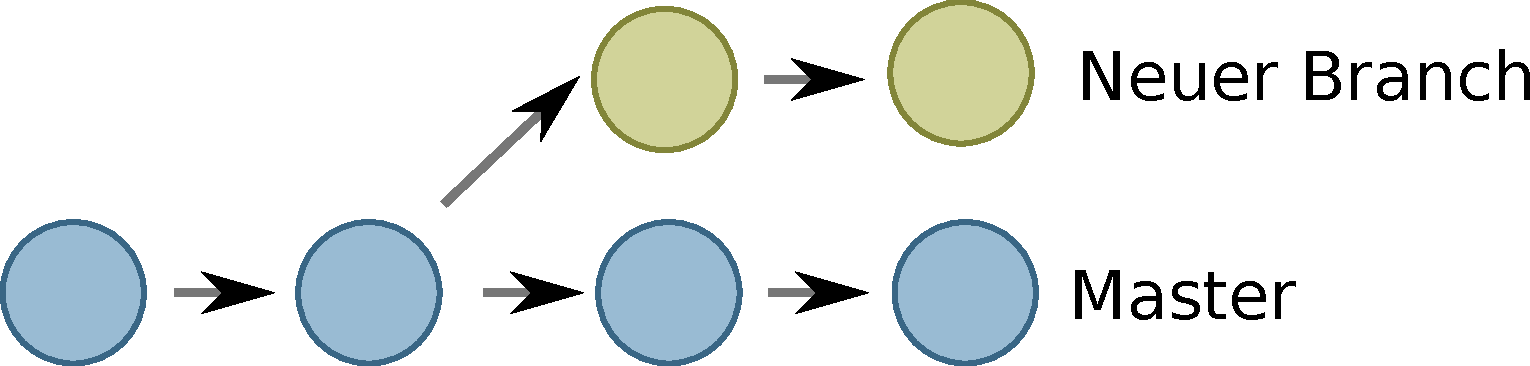
\includegraphics[width=7cm]{bilder/branch.pdf}
\end{center} 
%    \caption{}
%    \label{fig:awesome_image}
\end{figure}

Will man jedoch einen neuen Branch erstellen, um beispielsweise ein neues Feature erst einmal für sich zu programmieren, so benutzt man
\begin{verbatim}
git checkout -b neuer_branch
\end{verbatim}
Wobei \qmarks{neuer\_ branch} der Name des neuen Branches ist, den man erstellen will.

Um zum Master-Branch zurückzuwechseln, verwendet man \qmarks{git checkout master}.

Das Löschen eines Branches funktioniert mit
\begin{verbatim}
git branch -d neuer_branch
\end{verbatim}

Der Branch ist jedoch noch nicht entfernt verfügbar, sondern nur auf der lokalen Maschine.
Um den Branch anderen verfügbar zu machen, muss man ihn erst hochladen:
\begin{verbatim}
git push origin <branch>
\end{verbatim}

Um Änderungen zu aktualisieren, verwendet man hier ebenfalls \qmarks{git pull}.

Will man den aktuellen Branch mit einem anderen zusammenführen, so verwendet man den
\begin{verbatim}
git merge <branch>
\end{verbatim}
Befehl.

Git versucht in beiden Fällen die Änderungen automatisch zusammenzuführen.
Ist dies nicht möglich, so muss man die Änderung selbst durchführen.
Git meldet in diesem Fall Konflikte.
Sind diese Konflikte aufgelöst, so kann man sie wieder mit
\begin{verbatim}
git add <dateiname> 
\end{verbatim}
stagen.

Mit 
\begin{verbatim}
git diff <quell_branch> <ziel_branch>
\end{verbatim}
lassen sich die Unterschiede näher betrachten.

\subsubsection{Zurücksetzen}
\marginpar{Kada}

\begin{figure}[htb]
\begin{center}
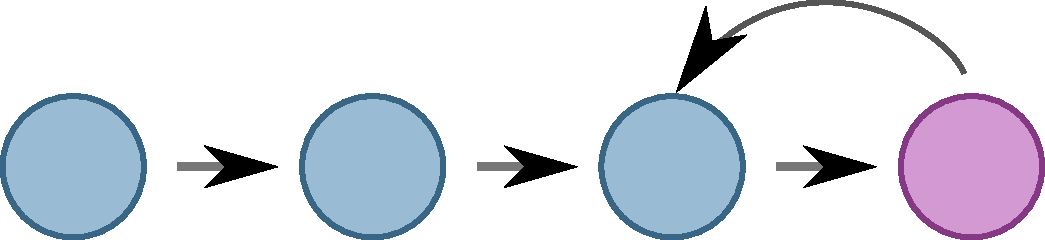
\includegraphics[width=7cm]{bilder/back.pdf}
\end{center} 
%    \caption{}
%    \label{fig:awesome_image}
\end{figure}
Für den den Fall, dass man lokale Änderungen wieder rückgängig machen möchte, kann man mit
\begin{verbatim}
git checkout --<filename>
\end{verbatim}
den Stand auf HEAD zurücksetzen lassen.

Sind die Änderungen bereits im Stage, so muss man sich eine Kopie aus dem entfernten Repository holen.
Die geschieht mit:
\begin{verbatim}
git fetch origin
git reset --hard origin/master
\end{verbatim}

\subsubsection{Forward}
\marginpar{Kada}

\begin{figure}[htb]
\begin{center}
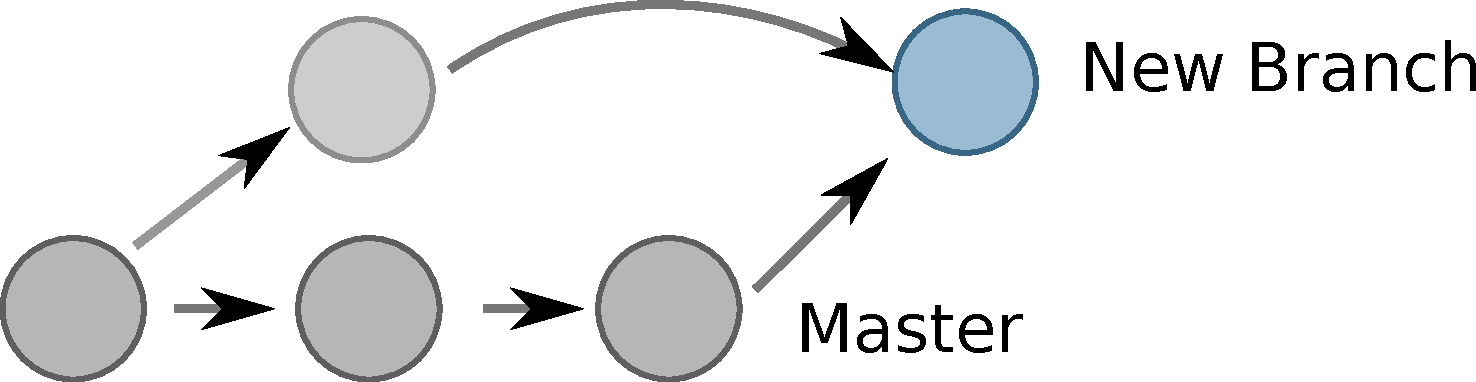
\includegraphics[width=7cm]{bilder/merge.pdf}
\end{center} 
%    \caption{}
%    \label{fig:awesome_image}
\end{figure}
\newpage

\section{Programmiersprache und Hilfsmittel}
\marginpar{Jan}

In diesem Abschnitt werden die programmiertechnischen Hilfsmittel beschrieben und erläutert.
Vor Beginn des einjährigen Projektes stand die Wahl der Programmiersprache zur Debatte.
Zur Auswahl standen C++ und Python, welche beide Vor- und Nachteile besaßen.
Größter Vorteil von Python ist die Kompaktheit, mit der Projekte konstruiert werden können.
Bei C++ stehen jedoch leistungsstarke Bibliotheken zur Verfügung, die neben Vorkenntnissen der Teilnehmer letztendlich den Ausschlag gaben.
% Anmerkung Marcel: War der eigentliche Grund nicht eher die Kenntnisse über die Sprachen? Python fast nicht bekannt und C++ mindestens bei der Hälfte der PG öfter benutzt. (evtl. waren da auch noch Einwände wegen Geschwindigkeit und C++-Python-Bindings?)

Zunächst wird kurz auf die Programmiersprache C++ und die benutze Entwicklungsumgebung, den Qt-Creator, eingegangen.
Zum Ende dieses Abschnittes wird die Bibliothek \textit{SeqAn} vorgestellt, welche zahlreiche Funktionen für die Behandlung von Datenstrukturen aus dem Bereich der Bioinformatik zur Verfügung stellt.
\subsection{C++}
\marginpar{Jan}
Die Programmiersprache C++ wurde von Bjarne Stroustrup entwickelt und erschien 1985 in der ersten Version.
Wie der Name schon andeutet, ist C++ eine Erweiterung der Programmiersprache C um verschiedene Aspekte, wie beispielsweise Klassen \citep{Stroustrup1996}.
Außerdem besteht eine Abwärtskompatibilität zu C, wodurch sich C-Code direkt ausführen lässt.
Nachteilig wirkt sich dadurch aber aus, dass sich viele Designnachteile auch in C++ wiederfinden.
Dazu gehört beispielsweise die Trennung in Headerdateien, welche vom sogenannten Präprozessor geladen werden, und dem eigentlichen Code.
Gemeinsames Designziel beider Sprachen ist aber die Effizienz, welche zum großen Teil durch die Speicherverwaltung erreicht wird.
Es wird kein \textit{Garbage-Collector} eingesetzt, wodurch der Programmierer mehr Kontrolle (aber auch Verantwortung) über das Programm erhält.

Dies steht im Gegensatz zu Java, wo der Aspekt der Plattformunabhängigkeit stärker wiegt als die Effizienz.
Die Unabhängigkeit ist bei C++ nicht (direkt) gegeben, da der Compiler für jedes System den systemspezifischen Maschinencode erzeugt.
Durch den Einsatz des Qt-Creators, der im nächsten Abschnitt beschreiben wird, haben wir eine einfache Möglichkeit, um die Unabhängigkeit über Umwege zu erreichen.

\subsection{Qt-Creator}
\marginpar{Jan}
Als Entwicklungsumgebung setzt unsere Projektgruppe den Qt-Creator ein.
Dieser wurde ursprünglich vom Qt-Projekt für die Entwicklung von plattformunabhängigen grafischen Oberflächen mit der Qt-Bibliothek entwickelt.
Es lassen sich jedoch auch allgemeine C++-Projekte damit entwickeln.

Die Plattformunabhängigkeit ist ein entscheidender Faktor, da alle drei großen Betriebssysteme, Windows, Mac OS und Linux, von den Teilnehmern des Projekts eingesetzt werden.
Wir ersparen uns durch die Nutzung außerdem Portierungsarbeiten, da die Qt-Bibliothek die Programmierung von Multithreading und grafischen Oberflächen vereinfacht.
Auch die Festlegung auf ein Zielsystem entfällt.

\subsection{SeqAn}
\marginpar{Benjamin}

SeqAn ist eine C++-Bibliothek zur Verarbeitung von biologischen Daten. Sie geht
auf ein Forschungsprojekt an der FU Berlin zurück und
stellt effiziente Algorithmen und Datenstrukturen zur Verfügung, die auf
Sequenzen arbeiten. Die Bibliothek ist in C++ implementiert und auf Effizienz
und Erweiterbarkeit optimiert, was durch die rigorose Verwendung von
Template-Metaprogrammierung erreicht wird. Dies stellt auch gleichzeitig den
größten Nachteil von SeqAn dar, da einiges an Einarbeitung erforderlich ist, um
mit dieser Programmierweise umgehen zu können.

Für die Projektgruppe hat sich SeqAn aus mehreren Gründen gegen andere
Bibliotheken durchgesetzt.

\begin{itemize}
	\item Unterstützung aller gängigen und von der Projektgruppe benötigten
          Dateiformate.
    \item Geschwindigkeit und Speicherverbrauch haben eine hohe Priorität.
	\item Sehr große Auswahl an Algorithmen mit dem sehr schnell
          Readmapper-Prototypen entwickelt werden können.
	\item Funktioniert auf vielen verschiedenen Plattformen, insbesondere
          auch unter Windows, was das Testen erleichtert.
\end{itemize}

Unser Readmapper benutzt SeqAn derzeit zur Ein- und Ausgabe von FASTA-,
FASTQ- und VCF-Dateien, zur Auswertung von Kommandozeilenoptionen und zur generellen
Behandlung von DNA-Strings. Hierbei haben sich die verschiedenen unterstützten
Alphabete wie DNA, DNA mit 'N' und IUPAC (siehe Abschnitt~\ref{sec:data:iupac}) als nützlich erwiesen.
Unsere Mapping- und Alignierverfahren nutzen derzeit die in der Bibliothek bereitgestellten Algorithmen nicht als Grundlage, da sie zu stark von den verbreiteten Verfahren, die in SeqAn implementiert sind, abweichen.
